%        File: TDDD14-lecture-notex.tex
%     Created: Mon Apr 04 10:00  2016 C
% Last Change: Mon Apr 04 10:00  2016 C
%
\documentclass[a4paper]{article}
\usepackage[utf8]{inputenc}
\usepackage{float}
\usepackage{graphicx}
\usepackage{hyperref}
\usepackage{amssymb}
\usepackage{mathtools}
\newtheorem{definition}{Definition}
\newtheorem{lemma}{Lemma}
\newtheorem{theorem}{Theorem}
\newtheorem{example}{Example}
\title{Lecture Notes\\TDDD14}
\author{Pontus Persson}
\date{VT-16}

\begin{document}
\maketitle
\tableofcontents
\marginpar{Lecture 1\\2016-04-04}
\section{Introduction}
Course questions:
\begin{itemize}
    \item What is a computer?
    \item What is their computational power?
    \item Programming languages
    \item Compilers
\end{itemize}
Some answers:
\begin{itemize}
    \item Different computational models leads to different computational powers
    \item Yes, there are problems which a computer can not solve
\end{itemize}
\subsection{Automata}
\textbf{Course backbone:} Automata\\
We use them to define formal languages and more importantly, computational models.
\\Many applications:
\begin{itemize}
    \item Artificial intelligence
    \item Vending machines
    \item Traffic lights, turnstile
    \item Video games
\end{itemize}
\begin{figure}[H]
    \centering
    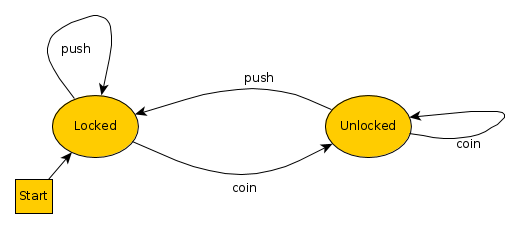
\includegraphics[width=0.9\textwidth]{turnstile.png}
    \caption{Turnstile Automata}
    \label{fig:turnstile}
\end{figure}
We treat mainly three types of automata:
\begin{enumerate}
    \item Finite memory (finite automata, FAs, e.g. turnstile)
    \item Infinite memory with restricted access (push-down automata, PDAs)
    \item Infinite memory without restricted access.
\end{enumerate}
\subsection{Some terminology}
Should be familiar with:
\begin{itemize}
    \item Sets and operations with sets
    \item Functions
    \item Relations
    \item Cartesian product
    \item Some sense of order and partial orders
    \item Equivalence relation
    \item Graphs and trees
    \item Binary and decimal repr. of numbers
\end{itemize}
\section{Basic definitions}
\begin{definition}
    A \textbf{decision problem} is a function with a one bit output: ``yes'' or ``no''.\\
    To specify a decision problem, we need two things:
    \begin{itemize}
        \item The set A of possible inputs
        \item The subset $B\subseteq A$ of ``yes'' instances
    \end{itemize}
\end{definition}
\begin{example}
    Given n, is n odd? Is a decision problem\\
    $A=\mathbb{N}$, $B=\left\{ n\in\mathbb{N} \middle| n\equiv 1 (mod 2) \right\}$\\
\end{example}
\begin{example}
    Given a,b. What is the greatest common divisor? Is not a decision problem.
\end{example}
In this course: an input is always a string of some alphabet.
\begin{definition}
    An \textbf{alphabet} is any finite set.\\
    We call the elements of this set symbols or letters. An alphabet is typically
    denoted with $\Sigma, \Gamma$. Symbols are often denoted with $a,b,c,\ldots$
\end{definition}
\begin{definition}
    A \textbf{string} over $\Sigma$ is any finite-length sequence of elements of $\Sigma$.\\
    We usually denote strings x,y,z,w,u,v,\ldots
\end{definition}
\begin{example}
    If $\Sigma=\left\{ a,b \right\}$, then ``aabab'' is a string over $\Sigma$ of length 5.
\end{example}

\begin{definition}
    The \textbf{length} of a string x is the number of symbols in x.\\
    Denoted by $|x|$.
\end{definition}
\begin{definition}
    The \textbf{null string} of \textbf{empty string} is denoted by $\varepsilon$.\\
    $|\varepsilon|=0$
\end{definition}
\begin{definition}
    Some terminology.
    \begin{itemize}
        \item $a^n$ A string of a's of length n ($a^5=aaaaa$, $a^0=^{def}\varepsilon$)
        \item The set of all string over $\Sigma$ is denoted by $\Sigma^*$.
        \item $\emptyset^*=\left\{ \varepsilon \right\}$
        \item If $\Sigma$ is non-empty then, $\Sigma^*$ is an infinite set of
            finite-length strings.
        \item Note: $\emptyset,\left\{ \varepsilon \right\}, \varepsilon$ are three
            \textbf{different} things.
    \end{itemize}
\end{definition}
\begin{definition}
    \textbf{Concatenation} takes two strings and x,y and creates a new string xy
            by putting them together end to end. xy is called the concatenation of x and y.\\
            \textbf{Note:} $xy \neq yx$ in general.
            \begin{itemize}
                \item Concatenation is associative: $(xy)z=x(yz)$
                \item $\varepsilon$ is an identity for concatenation $\varepsilon x=x\varepsilon = x$
                \item $|xy|=|x|+|y|$
                \item $a^ma^n=a^{m+n}$
            \end{itemize}
\end{definition}
\begin{definition}
    We write $x^n$ for the string obtained by concatenating n copies of x.
\end{definition}
\begin{definition}
    If $a\in\Sigma$ and $x\in\Sigma^*$ we write $\#a(x)$ for the number
            of a's in x
\end{definition}
\begin{definition}
    A \textbf{prefix} of a string x is an initial substring of x.
\end{definition}
\begin{definition}
    A \textbf{suffix} of a string x is an ending substring of x.
\end{definition}
\begin{definition}
    The \textbf{complement} in $\Sigma^*$, $A\subseteq\Sigma^*$ is denoted by
    $~A=\left\{ x\in\Sigma^* \middle| x\notin A \right\}$, we denote it by $\hat{A}$.
\end{definition}
\begin{definition}
    Set concatenation $A,B\in\Sigma^*$, $AB=\left\{ xy \middle | x\in A, y\in B \right\}$
\end{definition}
\begin{definition}
    Any subset $A\subseteq \Sigma^*$ is called a \textbf{language}.
\end{definition}
\section{States and Transitions}
\marginpar{Lecture 2\\2016-04-06}
Intuitively, a \textbf{state} is a snapshot of a system (automata). A state gives
all relevant information necessary to determine how the system will evolve from
that point on.
\\\textbf{Transitions} are changes of state, they can happen spontaneously, or in response
to external inputs.
\\A system that consists of only finitely many states and transitions among
them is called a \textbf{finite state system}.
\\We will model these by a model called \textbf{finite automaton}.
\subsection{Deterministic finite automaton (DFA)}
Formally a \textbf{deterministic finite automaton} (DFA) is a structure.
\begin{align*}
    M=(Q,\Sigma,\delta,s,F)
\end{align*}
Where:
\begin{itemize}
    \item $Q$ is a finite set of states
    \item $\Sigma$ is a finite set, the input alphabet
    \item $\delta : Q\times\Sigma\rightarrow Q$ is the transition function
    \item $s\in Q$ the start state
    \item $F\subseteq Q$ is the set of final states (accept states)
\end{itemize}

\begin{example}
    3.1 in the book.\\
    a)\\
\begin{align*}
    Q&=\left\{ 0,1,2,3 \right\}\\
    \Sigma&=\left\{ a,b \right\}\\
    \delta(0,a)&=1\\
    \delta(1,a)&=2\\
    \delta(2,a)&=\delta(3,a)=3\\
    \delta(q,b)&=q,\mbox{, }q\in Q\\
    s&=0\\
    F&=\left\{ 3 \right\}
\end{align*}
b) (table representation)
\begin{table}[H]
    \centering
    \begin{tabular}{l|l l}
        & a & b\\\hline
        0 & 1 & 0\\
        1 & 2 & 1 \\
        2 & 3 & 2 \\
        3F & 3 & 3
    \end{tabular}
    \caption{Table representation}
\end{table}
c) (transition diagram)
\begin{figure}[H]
    \centering
    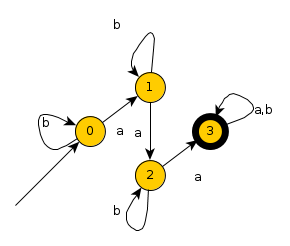
\includegraphics[width=0.8\textwidth]{transition-diagram.png}
    \caption{Transition diagram}
\end{figure}
This automaton excepts all strings/languages containing at least three ``a''s.\\
\end{example}
\subsubsection{State acceptance}
We define a function
\begin{align*}
    \hat{\delta}&: Q\times\Sigma^*\rightarrow Q
\end{align*}
by induction on the length of the string x:
\begin{align*}
    \hat{\delta}(q,\varepsilon)&=q\\
    \hat{\delta}(q,xa)&=\delta(\hat{\delta}(q,x),a)
\end{align*}
$\hat{\delta}$ is the multi-step version of $\delta$. $\delta$ and $\hat{\delta}$
agree on string of length one:
\begin{align*}
    \hat{\delta}(q,a)&= \hat{\delta}(q, \varepsilon a)\\
    &=\delta(\hat{\delta}(q,\varepsilon),a)\\
    &=\delta(q,a)
\end{align*}
A string $x$ is said to be accepted by the automaton $M$ if:
\begin{align*}
    \hat{\delta}(s,x)&\in F
\end{align*}
and rejected by automaton $M$ if:
\begin{align*}
    \hat{\delta}(s,x)\notin F
\end{align*}
where $s$ is the start state and $F$ is the set of final states of $M$.
\subsubsection{Accepted languages}
The set or language accepted by $M$ is the set of all strings accepted by $M$
, and is denoted $L(M)$.
\begin{align*}
    L(M)=\left\{ x\in\Sigma^*\middle | \hat{\delta}(s,x)\in F \right\}
\end{align*}
A language $A\subseteq \Sigma^*$ is said to be \textbf{regular} if $A=L(M)$
for some finite automaton $M$.\\
\textbf{NOTE:} The language accepted by the finite automaton from the example
above is regular.
\begin{example}
    3.2 in the book.\\
    \begin{align*}
        L_2&=\left\{ xaaay \middle | x,y\in \left\{ a,b \right\}^* \right\}\\
        &=\left\{ x\in\left\{ a,b \right\}^* \middle | x 
        \mbox{ contains a substring of three consecutive a's} \right\}
    \end{align*}\\
    \begin{table}[H]
        \centering
        \begin{tabular}{r|l l}
            & a & a
            \\\hline
            $\rightarrow$0 & 1 & 0\\
            1 & 2 & 0\\
            2 & 2 & 0\\
            3F & 3 & F
        \end{tabular}
    \end{table}
    \begin{figure}[H]
        \centering
        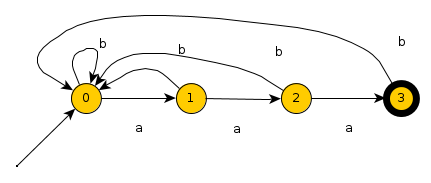
\includegraphics[width=0.9\textwidth]{example3-2.png}
    \end{figure}
\end{example}
\begin{example}
    \begin{align*}
        L_3=\left\{ x\in\left\{ 0,1 \right\}\middle | \mbox{x represents a multiple of three in binary} \right\}
    \end{align*}
    Here is an automaton that accepts $L_3$:
    \begin{table}[H]
        \centering
        \begin{tabular}{r|l l}
            & 0 & 1\\\hline
            $\rightarrow$0F & 0 & 1\\
            1 & 2 & 0\\
            2 & 1 & 2
        \end{tabular}
    \end{table}
    \begin{figure}[H]
        \centering
        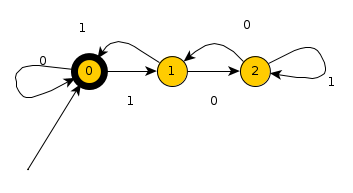
\includegraphics[width=0.9\textwidth]{example4.png}
    \end{figure}
    \textbf{Observations:}
    \begin{enumerate}
        \item append 0: multiply by 2
        \item append 1: multiply by 2 and add 1
    \end{enumerate}
    If the number represented by the string that is scanned so far is:
    \begin{itemize}
        \item $0 (mod 3)$
        \item $1 (mod 3)$
        \item $2 (mod 3)$
    \end{itemize}
    it will be in state 0, 1, 2 respectively.\\
    Property from Number Theory:
    \begin{align*}
        x,y,z &\in \mathbb{Z}\\
        \mbox{if } \\
        x&\equiv y (mod z)\\
        \mbox{then } \\
        ax+b &\equiv ay+b (mod x),\forall a,b\in\mathbb{Z}
    \end{align*}
Show that the transition will be true for all combinations of states and inputs.
\end{example}
\subsection{Determinism}
Determinism: At any step during the execution it is completely determined
what the system does next (depending on current state and input).
\subsection{Non-determinism}
Non-determinism: During the execution it is not always determined what to do
next, that means that a choice has to be made (a choice that does not depend
on current state nor input).
\subsection{Non-deterministic automaton (NFA)}
In a non-deterministic automaton the next state is not necessarily uniquely
determined by current state and input. There may be one, many, or even zero
next states. NFAs may have several start states.
\\An NFA works as a DFA, but in addition, whenever the next state is not uniquely
determined, it ``guesses'' what next state to assume.
\\Obviously, different guesses may lead to different computation paths and outcomes
(accept vs. reject).
\begin{figure}[H]
    \centering
    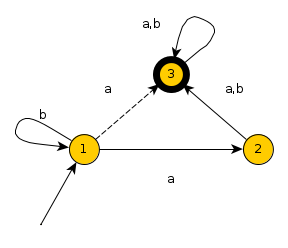
\includegraphics[width=0.6\textwidth]{nfa.png}
    \caption{An example of an NFA}
\end{figure}
\subsubsection{NFA acceptance}
An NFA is said to accept an input $x$ if at least one possible computation
path of input $x$ starting from at least one of the start states leads to a
final state.
\begin{example}
    \begin{figure}[H]
        \centering
        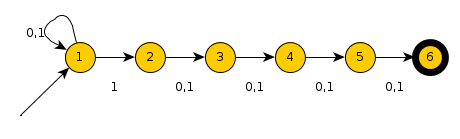
\includegraphics[width=0.9\textwidth]{nfa2.png}
        \caption{State diagram for example 7}
    \end{figure}
    Is an NFA because of the choice in state 1 and getting stuck in state 6 if
    there is input left.\\
    Input: 010111 can be accepted.\\
    Input: 100000 always rejected.
\end{example}
Can NFAs accept more languages than DFAs?\\
\textbf{NO!}\\
We will show how to construct for any NFA an equivalent DFA in the sense of
accepted language.
\subsubsection{NFA to DFA conversion}
\begin{example}
    5.1 in the book\\
    \begin{align*}
        A=\left\{ x\in\left\{ 0,1 \right\}^* \middle | 
        \mbox{the second symbol from the right is 1} \right\}
    \end{align*}
    \begin{figure}[H]
        \centering
        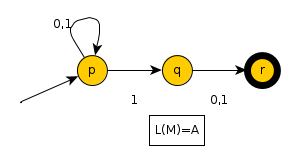
\includegraphics[width=0.6\textwidth]{example5-1-1.png}
        \caption{NFA example}
    \end{figure}
    \begin{table}[H]
        \centering
        \begin{tabular}{r|l l}
            DFA & 0 & 1 \\\hline
            $\emptyset$ & $\emptyset$ & $\emptyset$\\
            $\left\{ q \right\}$ & $\left\{ p \right\}$ & $\left\{ p,q \right\}$\\
            $\left\{ p \right\}$ & $\left\{ r \right\}$ & $\left\{ r \right\}$\\
            $\left\{ r \right\}$ & $\emptyset$ & $\emptyset$\\
            $\left\{ p,q \right\}$ & $\left\{ p,r \right\}$ & $\left\{ p,q,r \right\}$\\
            $\left\{ p,r \right\}$ & $\left\{ p \right\}$ & $\left\{ p,q \right\}$\\
            $\left\{ r,q \right\}$ & $\left\{ r \right\}$ & $\left\{ r \right\}$\\
            $\left\{ p,q,r \right\}$ & $\left\{ p,r \right\}$ & $\left\{ p,q,r \right\}$
        \end{tabular}
        \caption{All possible subsets we could be in}
    \end{table}
    Cross off all states not reachable when starting from the start state.
    \begin{figure}[H]
        \centering
        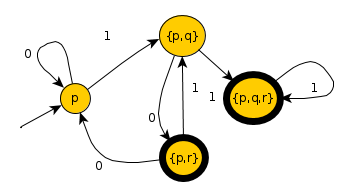
\includegraphics[width=0.7\textwidth]{example-5-2.png}
        \caption{DFA equivalent to previous NFA}
    \end{figure}
\end{example}
    \subsubsection{Formal definition of NFAs}
    An NFA is a five-tuble:
    \begin{align*}
        N&=\left( Q,\Sigma,\Delta,S,F \right)
    \end{align*}
    where:
    \begin{itemize}
        \item $S\subseteq Q$ is the set of start sets
        \item $\Delta: Q\time\Sigma^*\rightarrow 2^Q$
        \item All the rest as for the DFA definition
    \end{itemize}
    \textbf{Note:} $2^Q=\left\{ A\middle | A\subseteq Q \right\}$
        $\Delta(p,a)$ gives the set of all states that $N$ is allowed
        to move to from $p$ in one step ? input symbol $a$. The set $\Delta(p,a)$
        can be empty.\\
        $\Delta$ is called the transition function of $N$.
        \\We extent $\Delta$ to $\hat{\Delta}$ to the multistep version of $\Delta$.
        \begin{align*}
            \hat{\Delta}&:2^Q\times \Sigma^* \rightarrow 2^Q\\
            \hat{\Delta}(A,\varepsilon)&=A\\
            \hat{\Delta}(A,xa)&=\cup_{q\in\hat{\Delta}(A,x)}\Delta(q,a)
        \end{align*}
        For $A\subseteq Q$ and $x\in\Sigma^*$, $\hat{\Delta}(A,x)$ is the set
        of all states reachable under the input string $x$ from some state in $A$.
        \\\textbf{Note:} for $a\in\Sigma$
        \begin{align*}
            \hat{\Delta}(A,a)&=\cup_{p\in\hat{Delta}(A,\varepsilon)}\Delta(p,a)\\
            &=\cup_{p\in A}\Delta(p,a)
        \end{align*}
        The automaton $N$ is said to accept $x\in\Sigma^*$ if:
        \begin{align*}
            \hat{\Delta}(S,x)\cap F \neq \emptyset
        \end{align*}
        $L(N)$ is the set of all strings accepted by $N$.
        \begin{align*}
            L(N)=\left\{ x\in\Sigma^* \middle | \mbox{N accepts x} \right\}
        \end{align*}
        \textbf{Note:} Any DFA is equivalent to an NFA where:
        $\Delta(p,a) = \left\{ \delta(p,a) \right\}$.
        \begin{lemma}
            For any $x,y\in\Sigma^*$ and $A\subseteq Q$: $\hat{\Delta}(A,xy)=\hat{\Delta}(\hat{\Delta}(A,x),y)$
        \end{lemma}
        \subsubsection{The subset construction}
        Let
        \begin{align*}
            N=(Q_N,\Sigma,\Delta_N,S_N,F_N)
        \end{align*}
        be an arbitrary NFA.\\
        Let $M$ be the following DFA:
        \begin{align*}
            M=(Q_M, \Sigma, \delta_M, s_M, F_M)
        \end{align*}
        where:
        \begin{itemize}
            \item $Q_M = 2^Q$
            \item $\delta_M(A,a)=\hat{\Delta}_N(A,a)$
            \item $s_M=S_N$
            \item $F_M=\left\{ A\subseteq Q_N \middle | A \cap F_N \neq \emptyset \right\}$
        \end{itemize}

        \begin{lemma}
            For any $A\subseteq Q_N$ and $x\in\Sigma^*$
            \begin{align*}
                \hat{\delta}_M(A,x) = \hat{\Delta}_N(A,x)
            \end{align*}
            Proof via induction on the length of $x$.
        \end{lemma}

        \begin{theorem}
            The automata $M$ and $N$ accept the same language
            \begin{align*}
                x&\in L(M)\\
                \Leftrightarrow &\hat{\delta}_M(s_M,x)\in F_M\\
                \Leftrightarrow &\hat{\Delta}_N(S_M,x)\in F_M\\
                \Leftrightarrow &\hat{\Delta}_N(S_N,x)\in F_M\\
                \Leftrightarrow &\hat{\Delta}_N(S_N,x)\cap F_N \neq \emptyset\\
                \Leftrightarrow &x\in L(M)
            \end{align*}
        \end{theorem}
        \marginpar{Lecture 4\\2016-04-13}
        \subsection{$\varepsilon$-transition}
        We can have transitions without reading an input symbol.
        \begin{figure}[H]
            \centering
            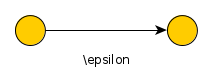
\includegraphics{epsilon.png}
            \caption{$\varepsilon$-transition}
            \label{fig:epstrans}
        \end{figure}
        \begin{definition}
            $NFA_\varepsilon$\\
            $N_\varepsilon = \left( Q,\Sigma, \Delta, S, F \right)$\\
            as NFA, but $\Delta: Q\times (\Sigma\cup \left\{ \varepsilon \right\}
            \rightarrow 2^Q$\\
            Note: $\Sigma$ never contains $\varepsilon$!
        \end{definition}

        For $A\subseteq Q$\\
        $C_\varepsilon(A)$ = all states reachable from some $q\in A$ via an
        $\varepsilon$-transition.
        \begin{definition}
            \begin{enumerate}
                \item $A\subseteq C_\varepsilon(A)$
                \item if $q\in C_\varepsilon(A)$, then $\Delta(q,\varepsilon)
                    \subseteq C_\varepsilon(A)$
                \item No other states are in $C_\varepsilon(A)$
            \end{enumerate}
        \end{definition}
        \begin{definition}
            \begin{align*}
            \hat{\Delta}&: 2^Q\times \Sigma^* \rightarrow 2^Q\\
            \hat{\Delta}(A,\varepsilon)&=C_\varepsilon(A)\\
            \hat{\Delta}(A,xa)&=C_\varepsilon(\cup_{q\in\hat{\Delta}(A,x)}\Delta
            (q,a)
        \end{align*}
        Note:
        \begin{align*}
            \hat{\Delta}(A,a)=C_\varepsilon(\cup_{q\in C_\varepsilon(A)}\Delta(q,a)
        \end{align*}
        \end{definition}
        \subsubsection{DFA from $\varepsilon$-NFA}
        From $N_\varepsilon = \left( Q_{N_c}, \Sigma, \Delta_{N_c}, S_{N_c}, F_{N_c} \right)$
        we construct the DFA $M=\left(Q_M, \Sigma, \delta_M, s_m, F_m\right)$.\\
        where:
        \begin{align*}
            Q_M&=2^{Q_{N_c}}\\
            s_M&=C_\varepsilon(S_{N_c}\\
            \delta_M(A,a)&=\hat{\Delta}(A,a)\\
            F_M&=\left\{ A\subseteq Q_{N_c}\middle | A\cap F_{N_c} \neq \emptyset \right\}
        \end{align*}
        You can prove via induction that $\hat{\delta}(s_M,x)=\hat{\Delta}(S_{N_c},x)$
        and then you show $L(N_c)=L(M).$.
        \begin{figure}[H]
            \centering
            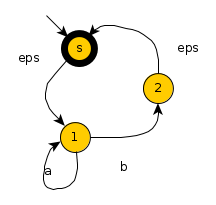
\includegraphics{nfaeps.png}
            \caption{$NFA_\varepsilon$}
            \label{fig:nfaeps}
        \end{figure}
        \begin{table}[H]
            \centering
            \begin{tabular}{r|l l|l|l| l l}
                & a & b & $\varepsilon$ & $C_\varepsilon$ & a & b\\\hline
                SF & $\emptyset$ & $\emptyset$ & 1 & $\left\{ 1 \right\}$ & $\left\{ s,1 \right\}$ & $\left\{  1,2,s\right\}$\\
                1 & 1 & 2 & $\emptyset$ & $\left\{ 1 \right\}$ &$\left\{ 1 \right\}$ & $\left\{ 1,2,S \right\}$\\
                2 & $\emptyset$ & $\emptyset$ & s & $\left\{ 2,s,1 \right\}$ & $\left\{ 1 \right\}$ & $\left\{ 1,2,s \right\}$
            \end{tabular}
        \end{table}
        \begin{figure}[H]
            \centering
            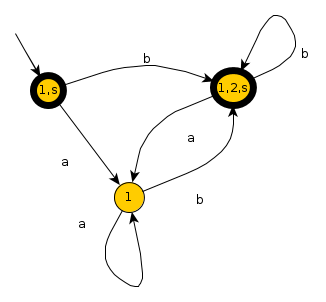
\includegraphics[width=0.8\textwidth]{dnanoeps.png}
            \caption{DFA from $NFA_\varepsilon$}
        \end{figure}
\section{Regular expressions}
\begin{definition}
    Given an alphabet $\Sigma$, the following are \textbf{regular expressions}:
    \begin{itemize}
        \item the empty set, denoted $\emptyset$
        \item the singleton set that contains the empty string 
            $\left\{ \varepsilon \right\}$, denoted by $\varepsilon$
        \item Any singleton set that contains a symbol from $\Sigma$
    \end{itemize}
\end{definition}
Let $X,Y$ be two regular expressions. The following operations are used to
produce more complex regular expressions:
\begin{itemize}
    \item concatenation, denoted $XY$.
    \item alternation (set unioun), denoted $X+Y$
    \item Kleene star, denoted $X^*$
\end{itemize}
Parentheses are allowed to reduce ambiguity. To reduce the use of parenthesis,
the Kleene star has highest priority, then concatenation and last alternation.
\textbf{Examples:}\\
$\Sigma = \left\{ a,b \right\}$
\begin{enumerate}
    \item $ab+a=\left\{ ab,a \right\}$
    \item $\left( a+b \right)^*=\left\{ \varepsilon,a,b,aa,ab,ba,bb,aaa,aab,\ldots \right\}$
    \item $\left(a+\varepsilon\right)b^*=\left\{ \varepsilon,a,b,ab,abb,abbb,bb,bbb,\ldots \right\}$
\end{enumerate}
Alteration and concatenation are associative, therefore parenthesis can be
omitted in the following cases:
\begin{itemize}
    \item $(a+b)+c=a+b+c$
    \item $(ab)c=a(bc)=abc$
\end{itemize}
Alternation is also commutative, concatenation is not.\\
Some transformation laws. Let $\alpha,\beta,\gamma$ be regular expressions.
\begin{align}
    \alpha+\emptyset &= \alpha\\
    \alpha+\alpha&=\alpha\\
    \varepsilon \alpha &= \alpha\\
    \alpha(\beta + \gamma) &= \alpha\beta + \alpha\gamma\\
    (\alpha+\beta)\gamma &= \alpha\gamma + \beta\gamma\\
    \varepsilon + \alpha\alpha^* &= \alpha^*\\
    (\alpha\beta)^*\alpha &= \alpha(\beta\alpha)^*\\
    (\alpha^*\beta)^* &= (\alpha+\beta)^* = \alpha^*(\beta\alpha^*)^*\\
    (\varepsilon+\alpha)^* &= \alpha^*\\
    \alpha\alpha^* &= \alpha^*\alpha
\end{align}
\subsection{Transform regular expression to $NFA_\varepsilon$}
\begin{itemize}
    \item $\emptyset\rightarrow \emptyset$
    \item $\varepsilon \rightarrow $ one state that is both start and final
    \item $a\rightarrow$ a start state and a final state connected by input $a$
\end{itemize}
\subsection{From regex to $NFA_\varepsilon$}
\subsubsection{Concatenation}
Concatenation of $X,Y$. Let $M_x$ ans $M_y$ be automata accepting $X$ and $Y$, respectively.\\
Let $F_x$ be the final states of $M_x$ and $S_y$ be the start states of $M_y$.
Introduce a new state $s,$ and introduce $\varepsilon$-transitions from every
state in $F_x$ to $s$ and from $s$ to every state in $S_y$. Make the states
in $F_x$ non-final states. The new automata is called $M_{XY}$.

\subsubsection{Alternation}
Alternation of $X,Y$. Simply define $M_{X+Y}$ as $M_X$ $M_Y$ ``together''
(is the sense that they are still disconnected). Same automata but, disconnected.

\subsubsection{Kleene star}
$X^*$. Introduce a new final start state s. $\varepsilon$-transitions
from s to all start states of $M_X$ and $\varepsilon$-transitions from all
final state of $M_X$ to s.\\
\textbf{Example:} $L=\left\{a^nb \middle | n\geq 0 \right\}= \left\{ b,ab,aab,aaab,\ldots \right\}$\\
$L^*=\left\{ w\in \left\{ a,b \right\}^* \middle | \mbox{w ends with b or }w=\varepsilon \right\}$
\subsection{From DFA to regexp}
\begin{figure}[H]
    \centering
    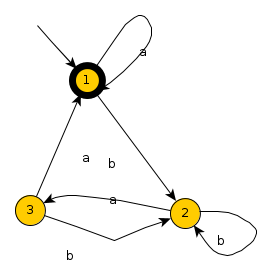
\includegraphics[width=0.7\textwidth]{dfa2regex.png}
    \caption{DFA}
\end{figure}
Associate a language to each state.\\
$A_i=L(q_i)=\left\{ x\in \Sigma^* \middle | \hat{\delta}(q_i,x)\in F \right\}=$
strings that move M from state $q_i$ to some final state.\\
Idea: express these languages in terms of each other, using regular expression-operations.
\begin{align}
    A_1&=aA_1+bA_2+\varepsilon\\
    A_2&=bA_2+aA_3\\
    A_3&=aA_1+bA_2
\end{align}
Then solve the equations! In particular we are interested in $A_1=L(M)$.
\\How to solve it? \textbf{Ardm's Theory}: \\Let $A,B$ languages, $\varepsilon \notin A$.
The equation $X=AX+B$ has the unique solution $X=A^*B$.
Eliminate $A_3$ using (13):
\begin{align*}
    A_2 &= bA_2 + a(aA_1+bA_2)\\
    &= bA_2 + aaA+1 + abA+2\\
    &= (ab+b)A_2+aaA_1\\
    \Leftrightarrow A_2 &= (ab+b)^*aaA_1\\
    \Rightarrow A_1 &= aA_1 + b(ab+b)^*aaA_1+\varepsilon \\
    &= (a+b(ab+b)^*aa)A_1+\varepsilon\\
    &= (a+b(ab+b)^*aa)^*
\end{align*}
\section{Equivalence relations}
Given $~\subseteq X\times X$ is an equivalence-relation if for any $x,y,x\in X$:
\begin{enumerate}
    \item $x\sim x$ (reflexive)
    \item $x\sim y \Rightarrow y\sim x$ (symmetric)
    \item $x\sim y$ and $y\sim z$ then $x\sim y$
\end{enumerate}
The equ-class of an $x\in X$ is the set $\left\{  y\in X \middle | y\sim x\right\}$.
It is denoted either by $\left[ x \right]_\sim$ or $x/\sim$.
\\The set of all equ-classes is denoted by $X/\sim$.\\
The number of equ-classes is called the index of $\sim$.

\section{DFA state minimization}
\begin{enumerate}
    \item Delete inaccessible states
    \item Collapse ``equivalent'' states
\end{enumerate}
Two states are equivalent when they have the same associated languages.\\
$p\in Q$, $L(p)=\left\{ x\in \Sigma^* \middle | \hat{\delta}(p,x) \in F \right\}$.
\subsection{Quotient construction}
$p \approx q \Leftrightarrow \forall x\in \Sigma^* (\hat{\delta}(p,x)\in F \Leftrightarrow \hat{\delta}(q,x) \in F) \Leftrightarrow L(p)=L(q)$.
\\\textbf{Note:} $\approx$ is an equ-relation.
\begin{lemma}
    $\approx$ is even a convergence relation with respect to $\delta$. That is,
    when $p\approx q$, then $\delta(p,a) \approx \delta(q,a) \forall a\in \Sigma$
\end{lemma}
Let $M=(Q,\Sigma, \delta, s, F$ be a DFA. Define $M/\approx = (Q', \Sigma, \delta', s', F')$.
\\Where:
\begin{align*}
    Q'&=\left\{ \left[ p \right]\middle | p \in Q \right\}\\
    \delta'(\left[ p \right], a) &= \left[ \delta(p,a) \right]\\
    s' &= \left[ s \right]\\
    F' &= \left\{ \left[ p \right] \middle | p\in F \right\}
\end{align*}

\begin{lemma}
    $p\in F$ iff $\left[ p \right]\in F'$.
\end{lemma}
\begin{lemma}
    $\hat{\delta}'(\left[ p \right],x)=\left[ \hat{\delta}(p,x) \right] \forall x\in \Sigma^*$
\end{lemma}
\begin{theorem}
        $L(M/\approx)=L(M)$\\
        \textbf{Proof:} 
        \begin{align*}
            x\in L(M/\approx) &\Leftrightarrow \hat{\delta}'(s',x)\in F'\\
            &\Leftrightarrow \hat{\delta}'(\left[ s \right],x)\in F' \\
            &\Leftrightarrow \left[ \hat{\delta}(s,x) \right] \in F'\\
            &\Leftrightarrow \hat{\delta}(s,x) \in F \\
            &\Leftrightarrow x\in L(M)
        \end{align*}
    \end{theorem}
    \subsection{Minimization example}
    How to minimize a DFA $M$? Detect inaccessible states, then construct $M/\approx$.
    \\Ho to determine $\approx$?\\
    Stepwise identify pairs if states that are definitely not equivalent.\\
    if $p  \not \approx q$, then there is a distinguishing string x,
    \begin{align*}
        \hat{\delta}(p,x)\in F \land \hat{\delta}(x,q) \notin F
    \end{align*}
    This observation can be extended to a correctness proof of the following algorithm
    to determine $\approx$.
    \begin{enumerate}
        \item Write down a table of all pars $\left\{ p,q \right\}$, initially unmarked
        \item Mark any $\left\{ p,q \right\}$ s.t. $p\in F \land q\not \in F$
            or $p\not\in F \land q\in F$
        \item Repeat until no more changes occur:
            \begin{itemize}
                \item If there exists an unmarked pair $\left\{ p,q \right\}$ s.t.
                    $\left\{ \delta(p,a), \delta(q,a) \right\}$ is marked
                    for some $a\in \Sigma$, then mark $\left\{ p,q \right\}$
            \end{itemize}
        \item When done, we have $p\approx q$ iff $\left\{ p,q \right\}$ is unmarked
    \end{enumerate}
    \begin{figure}[H]
        \centering
        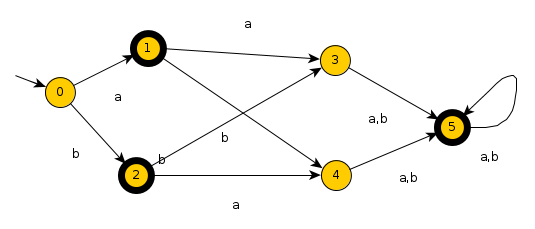
\includegraphics[width=0.9\textwidth]{unminimized.png}
        \caption{Unminimized DFA}
    \end{figure}
    \begin{table}[H]
        \centering
        \begin{tabular}{|l|l|l|l|l|l|}
            \hline
            0\\\hline
            x& 1\\\hline
            x& &2 \\\hline
            & x & x & 3 \\\hline
            & x & x & 4 \\\hline
            x & x1 & x & x & x & 5\\\hline
        \end{tabular}
        \caption{after step 1 and 2}
    \end{table}
    \begin{figure}[H]
        \centering
        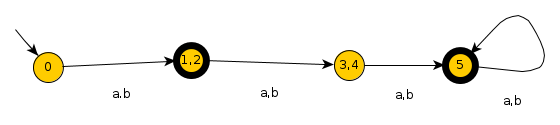
\includegraphics[width=0.9\textwidth]{minimized.png}
        \caption{minimized}
    \end{figure}
    \subsection{Myhill-Nerode Theorem}
    Let $L\subseteq \Sigma^*$ a language.\\
    Then L is regular if $\equiv_L$ is of infinite index.\\
    A DFA $M$ induces an equ-relation on $\Sigma^*$:
    \begin{align*}
        x\equiv_M y \Leftrightarrow \hat{\delta}(s,y)
    \end{align*}
    That is, $x \equiv_L$ if M goes on $x$ to the same state as on $y$.
    \\\textbf{Note:} $\equiv_M$ is an equ-relation. Every equ-class corresponds
    to a state of $M$.\\
    In the book $\equiv_M$ is called Myhill-Nerode relation.\\
    Also a language $L$ induces an equ-relation on $\Sigma^*$:
    \begin{align*}
        x\equiv_L y \Leftrightarrow \forall z\in \Sigma^*: xz\in L \Leftrightarrow yz\in L
    \end{align*}
    \subsubsection{Sketch of proof}
    ``$\Rightarrow$'' be L regular . Then there is a DFA M for L. We observe:
    \begin{itemize}
        \item whenever $x \equiv_M y$, then $x\equiv_L y$\\
            Therefore, any $\equiv_M$-equ-class is a subset of exactly on $\equiv_L$-equ-class.
        \item Since any $\equiv_L$-equ-class is a subset of $\Sigma^*$ and since
            $\equiv_M$ partitions $\Sigma^*$, any number of $\equiv_L$-equ-class
            must be in some $\equiv_M$-equ-class.
    \end{itemize}
    We conclude from these points that the number of $\equiv_L$-equ-classes can not be greater
    than the number of $\equiv_M$-equ-classes, which is the number of states of $M$,
    which is finite. $\Rightarrow \equiv_L$ is of finite index.\\
    ``$\Leftarrow$''. Let the number of $\equiv_L$-equ-classes be finite. We construct
    a DFA whose states ``are'' the $\equiv_L$-equ-clasees.
    \begin{itemize}
        \item start state: $\left[ \varepsilon \right]$
        \item a state $\left[ x \right]$ is final iff $\left[ x \right]$ contains
            some string from L
        \item $\delta(\left[ x \right], a) = \left[ xa \right]$
    \end{itemize}
    \begin{enumerate}
        \item Show that $\delta$ is well-defined\\
            (that is, $\delta(\left[ x \right],a)=\left[ ya \right] \forall y\in \left[ x \right]$
        \item Show that the DFA accepts exactly L
    \end{enumerate}
    \section{Slutenhetsegenskaper (closure properties)}
    $L_1,L_2$ reguljära språk. Är $L_1\cup L_2$ reguljärt? Is it true for all
    regular languages? In that case regular languages are closes under union.
    \begin{itemize}
        \item L regular $\Rightarrow$ $\sim L$ regular? $\sim L =$ complement\\
            Given an DFA A for L. Read x and ends in an end state $\Rightarrow$ $x\in L$\\
            New DFA $A'$ for $\sim L$ have the inverted end and non-end state compared to A.\\
            $\sim L$ is regular.
        \item $L_1,L_2$ regular $\Rightarrow$ $L_1 \cup L_2$ regular?\\
            Yes: $L_1=L(r_1),L_2=L(r_2),L_1\cup L_2 = L(r_1+r_2)$
        \item $L_1,L_2$ regular $\Rightarrow$ $L_1 \cap L_2$ regular? Yes!\\
            $L_1:a*b$ $L_2:ab*$ Build DFA where each state symbolizes being in a state in $L_1$ and $L_2$.\\
            Only states which contains end states from both languages are ok.\\
            $L_1\cap L_2: ab$
        \item Alternatively: $L_1\cap L_2 = \sim (\sim L_1 \cup \sim L_2)$
        \item Regular languages are closed under $\sim,\cup,\cap$ and under concatination and $*$.
    \end{itemize}

    \section{Homomorfismer}
    A homomorphism is a function $h:\Sigma^*\rightarrow \Gamma^*$.\\
    $h(xy)=h(h)h(y)$, $h(\varepsilon)=\varepsilon$\\
    It is enough to define $h:\Sigma \Rightarrow \Gamma^*$.\\
    \begin{itemize}
        \item $A\subseteq \Sigma^*:h(A)=\left\{ h(x) \middle | x\in A \right\}\subseteq \Gamma^*$
        \item $B\subseteq \Gamma^*:h^{-1}(B)=\left\{ x \middle | h(x) \in B \right\} \subseteq \Sigma^*$
    \end{itemize}
    Example: $\Sigma = \left\{ a,b,c,d,e \right\}$, $\Gamma = \left\{ p,q \right\}$.\\
    $h(a)=pp,h(b)=pq,h(c)=qq,h(d)=ppp,h(e)=qqq$.\\
    $A=\left\{ abc \right\},h(A)=\left\{ pppqqq \right\}$\\
    $B=\left\{ pppqqq \right\},h^{-1}(B)=\left\{ abc,de \right\}$\\
    L regular $\Rightarrow$ h,$h^{-1}$ regular.\\
    Regular languages are closed under homomorphism and inverse homomorphism.
    \section{Pumpinglemmat}
    \marginpar{Lecture 6\\2016-04-20}

\end{document}
